\section{Misura di portata mediante diaframma}
\subsection{Presentazione del banco prova, dati e richieste}
Viene assegnato un banco prova per misure di portata mediante diaframma normalizzato, rappresentato schematicamente in Fig.\ref{fig:schemabancoprova}. 

\begin{figure} [H]
	\centering
	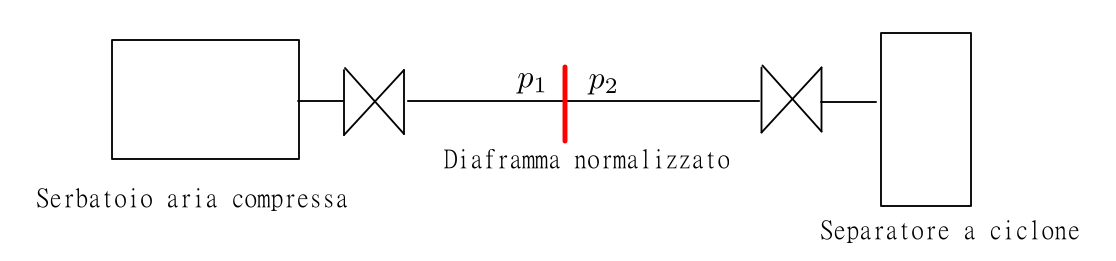
\includegraphics[width=\linewidth]{chapters/3-misuradiaframma/schemabancoprova}
	\caption{Schema del banco prova}
	\label{fig:schemabancoprova}
\end{figure}

In particolare, il separatore a ciclone opera nelle seguenti condizioni nominali:
\begin{itemize}
	\item fluido di lavoro (fase gas): aria;
	\item portata di aria nelle condizioni operative nominali: 96 Nm\textsuperscript{3}/h;
	\item pressione di lavoro: 4 bar;
	\item temperatura di lavoro (ambiente): 300 K.
\end{itemize}

Al fine di misurare la portata d'aria si sceglie di utilizzare un diaframma normalizzato conforme alla Norma UNI EN ISO 5167-1, rappresentato in Fig.\ref{fig:schemadiaframma} e con le seguenti caratteristiche: 
\begin{itemize}
	\item \gls{symb:D} = 42 mm;
	\item \gls{symb:d} = 9.94 mm;
	\item Prese di pressione sulle flange.
\end{itemize}

\begin{figure} [H]
	\centering
	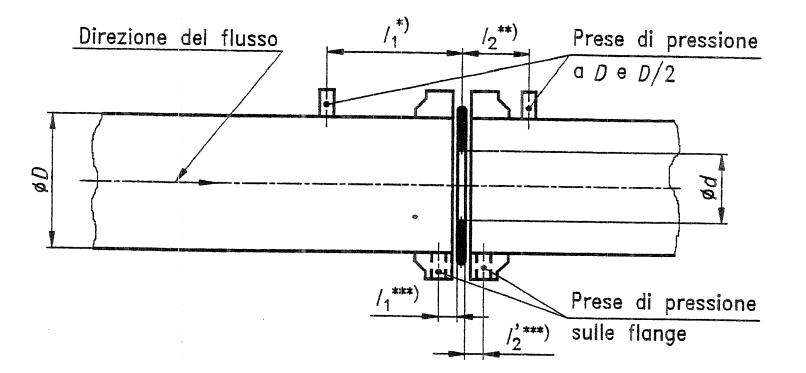
\includegraphics[width=0.7\linewidth]{chapters/3-misuradiaframma/schemadiaframma}
	\caption{Schema del diaframma (Fonte: UNI EN ISO 5167-1 Figura 5)}
	\label{fig:schemadiaframma}
\end{figure}

\paragraph{Richieste}
Si chiede di valutare la pressione minima di esercizio nel serbatoio di alimentazione e di indicare il trasduttore di pressione differenziale da usare sul banco prova per la misura di portata.


\subsection{Risoluzione}
Facendo riferimento a Fig.\ref{fig:schemabancoprova}, si denotino con \gls{symb:p}\textsubscript{1} e \gls{symb:p}\textsubscript{2} le pressioni (in Pa) a monte e a valle del diaframma. Si indichi con \gls{symb:T} la temperatura di esercizio (in K).

\paragraph{Ipotesi risolutive}
\begin{itemize}
	\item Le perdite di carico lungo il condotto e nelle valvole sono trascurate per mancanza di informazioni sull'impianto: di conseguenza \gls{symb:p}\textsubscript{1} è la pressione incognita del serbatoio di alimentazione, \gls{symb:p}\textsubscript{2} è la pressione operativa del separatore a ciclone.
	\item L'aria viene considerata come un gas perfetto, per cui \gls{symb:gamma} = \gls{symb:kappa} = 1.4, come indicato dalla Norma.
	\item Tutti i requisiti della Norma sono soddisfatti (Es. scabrosità del condotto, deformazione del diaframma, configurazione dello strumento).
	\end{itemize}

\paragraph{Riassunto dei dati e conversioni}
Si riporta un riassunto sintetico dei dati del problema, convertiti in unità del Sistema Internazionale dove necessario.
\begin{table}[H]
	\centering
	\begin{tabular}{c|c}
			\toprule
			\toprule
			\textbf{Dato} & \textbf{Valore} \\
			\midrule
			\midrule
			$D$ & 4.2e-2 m \\
			\midrule
			$d$ & 9.94e-3 m \\
			\midrule
			$p_2$ & 4.053e5 Pa\\
			\midrule
			$T_2$ & 300 K\\
			\midrule
			$\gamma $ & 1.4 \\
			\midrule
			$q_{\textit{vN}}$ & 96 Nm\textsuperscript{3}/h	\\
			\midrule
			$q_m$ & 0.0344 kg/s\\
			\bottomrule
			\bottomrule
	\end{tabular}
\end{table}
Al fine di convertire la portata volumetrica normalizzata in una portata massica si adotta la seguente espressione: 
\begin{equation}
	q_m = q_{\textit{vN}}\, \rho_N / 3600 
\end{equation}
con \gls{symb:rho}\textsubscript{N} = 1.293 kg/m\textsuperscript{3} la densità dell'aria a 273.15 K e 101325 Pa.

\paragraph{Svolgimento}
La Norma fornisce una serie di equazioni da utilizzare per la misura di portata massica, al cui interno sono definite delle quantità calcolate secondo la Norma stessa. Le equazioni risolventi del problema sono le seguenti:
\begin{equation}
	q_m=\frac{C}{\sqrt{1-\beta^4}}\, \epsilon_2 \,\frac{\pi}{4} \, d^2 \, \sqrt{2\Delta p \rho_2} \label{eq:portatamassica}
\end{equation}
\begin{equation}
	\epsilon_1= 1 - (0.41+0.35\beta^4) \, \frac{\Delta p}{\kappa p_1} \label{eq:epsilon1}
\end{equation}
\begin{equation}
	\epsilon_2=\epsilon_1 \, \sqrt{1+\frac{\Delta p}{p_2}} \label{eq:epsilon2}
\end{equation}
Le quantità qui presenti sono definite come:
\begin{itemize}
	\item \gls{symb:C} è ottenuto mediante opportuna espressione (Eq.);
	\item \gls{symb:beta} $ = d/D$;
	\item \gls{symb:rho}\textsubscript{2} $= p_2 / (RT_2) $, entrambe note, con $ R = 287 $ J/(kgK) per l'aria secca;
	\item $\kappa = \gamma = 1.4 $.
\end{itemize}
\gls{symb:C} viene calcolato con la seguente espressione:
\begin{equation}
	C=0.5959+0.0312\beta^{2.1}-0.1840\beta^8+0.0029\beta^{2.5} (10^6/Re_D)^{0.75}+0.0390L_1\beta^4(1-\beta^4)^{-1}-0.0337L_2'\beta^3 \label{eq:C}
\end{equation}
dove le quantità $L_1,\,L_2'$ sono calcolate in base alla Norma, mentre 